\newpage

\section{Scoring with Predicted Secondary Structure}

The previous tests were all done with secondary structure information gathered via \ac{DSSP} from the three-dimensional structure information. 
Homology prediction is a procedure commonly used for protein sequences for which the three-dimensional structure is unknown.
Furthermore, gaining knowledge about the homology is used to improve methods for determining the proteins tertiary structure.

\begin{figure}[!b]
	\begin{center}
		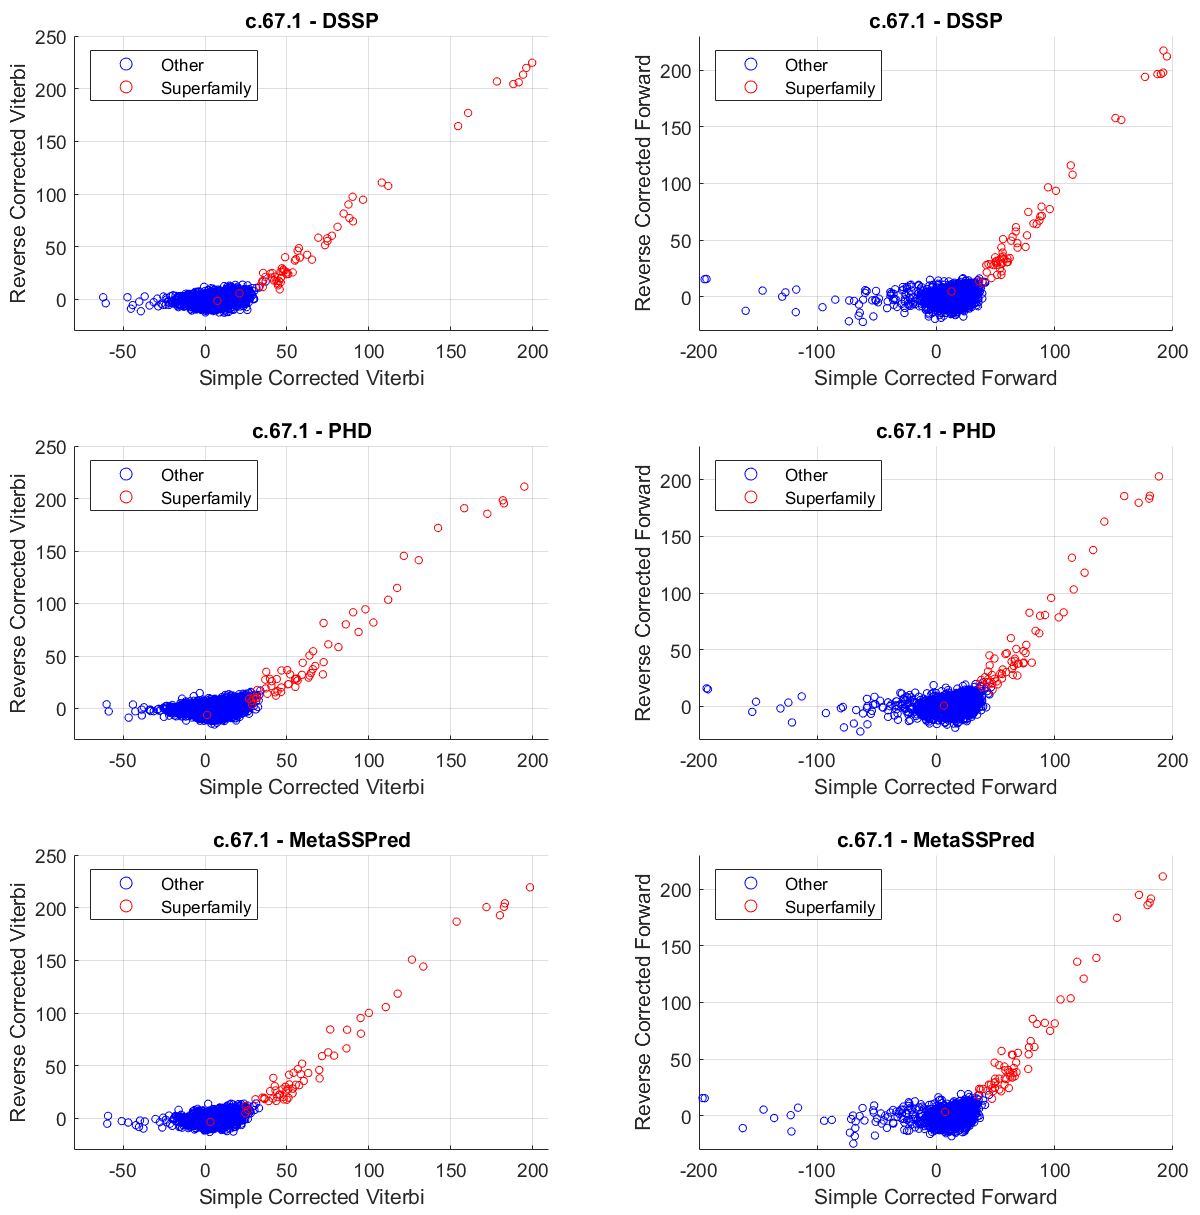
\includegraphics[width=0.97\textwidth]{fig/SS_NE}
	\end{center}
	\caption[Comparision of the different secondary structure estimation methods.]{Comparison of the different secondary structure estimation methods on \acs{MSA} c.67.1. }
	\label{fig:scattBssp}
\end{figure}

The following scatterplots in Figure \ref{fig:scattBssp} compare the results from the different methods of  secondary structure determination on the \ac{MSA} \texttt{c.67.1}. All plots show the simple-corrected scores on the horizontal axis and the reverse-corrected scores on the vertical axis.
 The first row is the reference plot with the secondary structure obtained from \ac{DSSP}.
 The structures for the second and third rows are predicted with \ac{PHD} and MetaSSPred, respectively.  
As in the previous sections, the method \texttt{M2\_025\_1\_3} is used for training the \ac{pHMM} and the test database is scored against it. 
For the \mbox{reverse-corrected} scores, the \ac{PCA} between the scores with and without secondary structure is used. Both the Viterbi scores on the left and the forward scores on the right show a slight decline. Even though the scores in the transition region between the superfamily and the other classes move closer to one another, there is still an outstanding improvement over the scores without secondary structure. This is also apparent in the \ac{ROC} curve in Figure \ref{fig:rocSS} based on the forward scores from Figure \ref{fig:scattBssp} and their associated primary-structure-only scores.

\begin{figure}[H]
	\begin{center}
		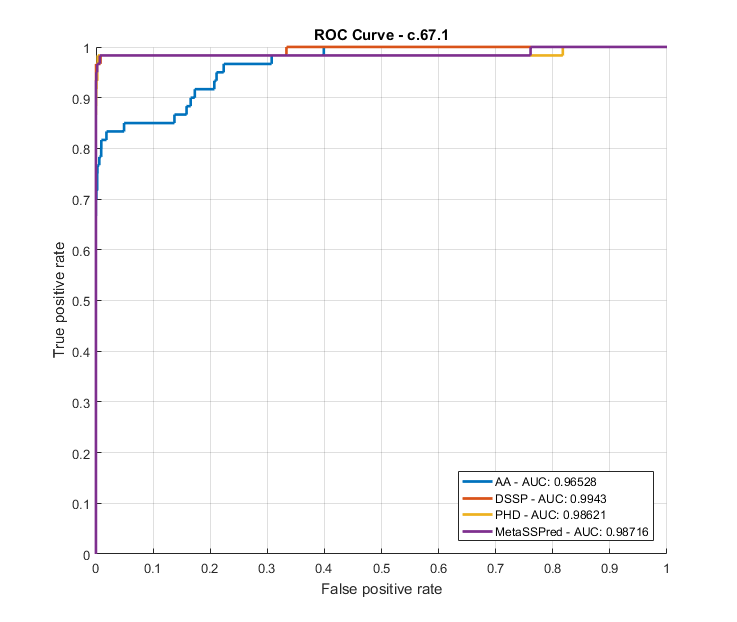
\includegraphics[width=0.8\textwidth]{fig/SSAuc}
	\end{center}
	\caption{\acs{ROC} curves comparing different secondary structure determination methods.} 
	\label{fig:rocSS}
\end{figure}